\documentclass[8pt]{beamer}

\usetheme[numbering=fraction, progressbar=foot, block=fill]{metropolis}
%\usecolortheme{seahorse}

\makeatletter
\setlength{\metropolis@titleseparator@linewidth}{1pt}
\setlength{\metropolis@progressonsectionpage@linewidth}{2pt}
\setlength{\metropolis@progressinheadfoot@linewidth}{2pt}
\makeatother

\usepackage{appendixnumberbeamer}
\usepackage{booktabs}
\usepackage{pgfplots}
\usepackage{tikz}
\usepackage{multicol}
\usepackage{changepage}
\usepackage{hyperref}
\usepackage{makecell}
\usepackage{multirow}
\usepackage{arydshln}
\usepackage{mathtools}
\usepackage{graphicx}
\usepackage{bm}
\usepackage{cancel}
\usepackage[document]{ragged2e}
\usepgfplotslibrary{dateplot}
\usepackage{xspace}

\newcommand{\themename}{\textbf{\textsc{metropolis}}\xspace}

% ================== Customization
\definecolor{mygreen}{RGB}{40,85,175} %Dark green
\definecolor{myred}{RGB}{153,26,0} %Dark red
\definecolor{myblue}{RGB}{66,98,163} %Dark blue
\definecolor{mycolor}{RGB}{66,98,163}

\setbeamercolor{background canvas}{bg=white}

%\setbeamertemplate{blocks}[rounded][shadow=false]

% ================== Title page
\title{Search for dark matter production in association with a single top quark or a top quark pair in the dilepton final state at $\sqrt{s} = $ 13 TeV}
%\subtitle{The subtitle goes here}
%\date{\today}\newcommand{\themename}{\textbf{\textsc{metropolis}}\xspace}

% ================== Customization
\definecolor{mygreen}{RGB}{40,85,175} %Dark green
\definecolor{myred}{RGB}{153,26,0} %Dark red
\definecolor{myblue}{RGB}{66,98,163} %Dark blue
\definecolor{mycolor}{RGB}{66,98,163}

\setbeamercolor{background canvas}{bg=white}

%\setbeamerfont{institute}{series=\bfseries,parent=structure}
\setbeamerfont{institute}{size=\large}
\setbeamerfont{author}{size=\normalsize}
\setbeamerfont{date}{size=\normalsize}
%\setbeamertemplate{frame footer}{\footnotesize \insertshortauthor~(\insertshortinstitute)}
\setbeamerfont{page number in head/foot}{size=\small}
\setbeamerfont{frametitle}{size=\normalsize}

\newcommand{\backupbegin}{
   \newcounter{finalframe}
   \setcounter{finalframe}{\value{framenumber}}
}
\newcommand{\backupend}{
   \setcounter{framenumber}{\value{finalframe}}
}

%\setbeamertemplate{blocks}[rounded][shadow=false]

%\subtitle{The subtitle goes here}
%\date{\today}
%\date{}
%\author{\justifying Afiq Anuar, Alexander Grohsjean, Christian Schwanenberger, Dominic Stafford, Nicole Stefanov (1), Kristian Hahn, Kevin Sung (2), Pablo Martinez Ruiz Del Arbol, J\'{o}natan Piedra,  \textbf{C\'{e}dric Prieels (3)}, Deborah Pinna, Victor Shang (4)}
%\institute{\textbf{\textbf{January 8th 2021}} \\ 
%\begin{multicols}{2}
%\normalsize{(1) DESY} \\
%(2) NorthWestern University \\
%(3) Instituto de Fisica de Cantabria \\
%(4) University of Wisconsin
%\end{multicols}}
%
%\titlegraphic{
%   \tikz[overlay,remember picture]
%       \node[at=(current page.south east), anchor=south east] {
%           
\includegraphics[height=1cm]{figs/desy.png}\hspace{18pt}
\includegraphics[height=1.1cm]{figs/northwestern.png}\hspace{18pt}
\includegraphics[height=0.9cm]{figs/ifca.jpg}\hspace{18pt}
\includegraphics[height=1cm]{figs/wisconsin.png}\hspace{18pt}
\includegraphics[height=1cm]{figs/cms.jpg}
%       };
%}

\date{\vspace{-3pt}February 9th 2022}
\author{Pablo Mart\'{i}nez Ru\'{i}z del \'{A}rbol, J\'{o}natan Piedra Gomez, \textbf{C\'{e}dric Prie\"{e}ls}}
\institute{Thesis Endorsement - Answer to questions \\ Instituto de F\'{i}sica de Cantabria}

\titlegraphic{
   \tikz[overlay,remember picture]
       \node[at=(current page.south east), anchor=south east] {
           
\includegraphics[height=1.0cm]{figs/ifca_final.png}\hspace{18pt}
\includegraphics[height=1.2cm]{figs/uc.jpg}\hspace{8pt}
\includegraphics[height=1.4cm]{figs/csic.jpg}\hspace{8pt}
\includegraphics[height=1.2cm]{figs/maetzu.png}\hspace{8pt}
\includegraphics[height=1.2cm]{figs/cms.jpg}
       };
}

% ================== Document
\begin{document}

\maketitle

\begin{frame}{Low BDT region large discrepancies}
\justifying
\begin{block}{\centering Worst cases}\end{block} \vspace{-10pt}
\begin{figure}[htbp]
\centering
\begin{minipage}[b]{.49\textwidth}
\vspace{-5pt}
\begin{block}{\centering Scalar 100 GeV}\end{block}
\begin{center}
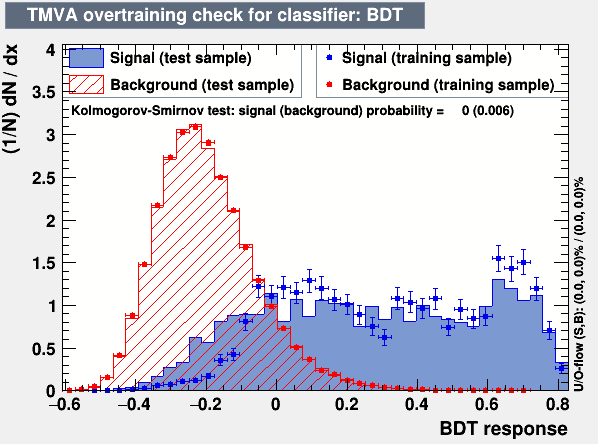
\includegraphics[width=5.2cm, height=3.5cm]{figs/overtraining_scalar100_TTbar.png}
\end{center}
\end{minipage}
\begin{minipage}[b]{.02\textwidth}\end{minipage}
\begin{minipage}[b]{.49\textwidth}
\vspace{-5pt}
\begin{block}{\centering Pseudo 100 GeV}\end{block}
\begin{center}
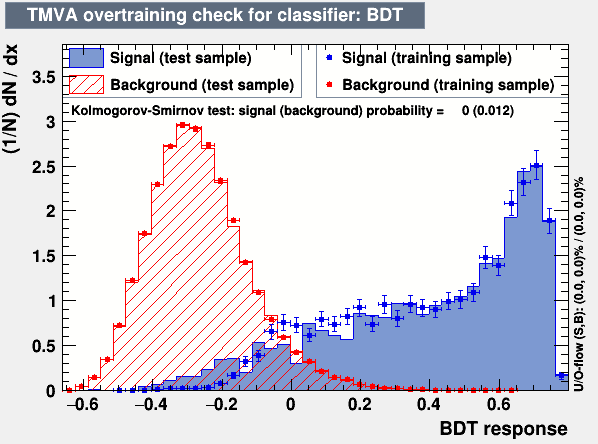
\includegraphics[width=5.2cm, height=3.5cm]{figs/overtraining_scalar500_TTbar.png}
\end{center}
\end{minipage}
\end{figure}

"You showed that signal in the low BDT region has large
data/simulation disagreement. This should be investigated. In addition,
it would be good to see the overtraining plots in log-scale so that we
ensure there is no large further disagreement in the tails of the
background in the high BDT region."
\end{frame}

\begin{frame}{Low BDT region large discrepancies}
\justifying
We first of all produced the exact same plots in log scale, as required. \vfill

\begin{figure}[htbp]
\centering
\begin{minipage}[b]{.49\textwidth}
\vspace{-5pt}
\begin{block}{\centering Scalar 100 GeV}\end{block}
\begin{center}
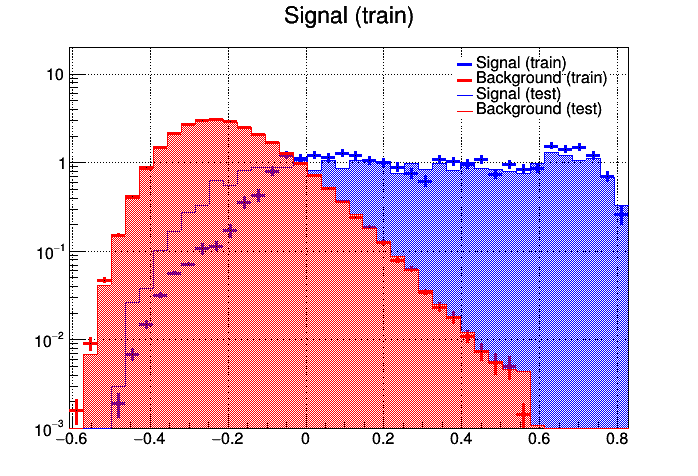
\includegraphics[width=5.2cm, height=3.5cm]{figs/log_scalar_overtraining_100GeV_TTbar.png}
\end{center}
\end{minipage}
\begin{minipage}[b]{.02\textwidth}\end{minipage}
\begin{minipage}[b]{.49\textwidth}
\vspace{-5pt}
\begin{block}{\centering Pseudo 100 GeV}\end{block}
\begin{center}
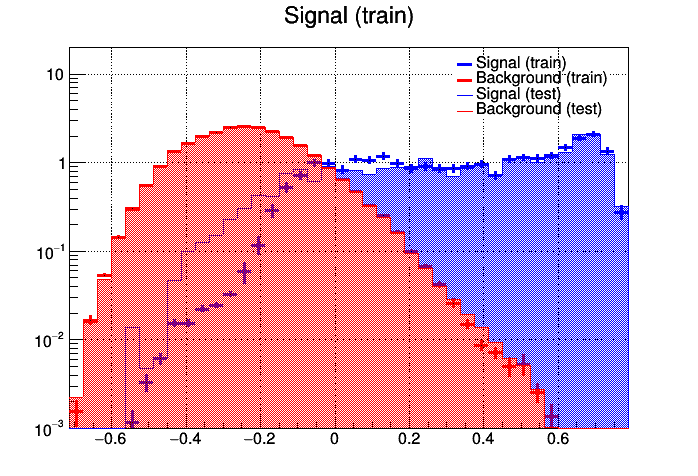
\includegraphics[width=5.2cm, height=3.5cm]{figs/log_pseudo_overtraining_100GeV_TTbar.png}
\end{center}
\end{minipage}
\end{figure}

These plots comfort us in the fact that no sign of test/train discrepancy is observed for the background samples, even in the tail. \vfill
\end{frame}


\begin{frame}{Low BDT region large discrepancies}
\justifying
%For the training process, both the $t/\bar t$ and $t \bar t$+DM are mixed together, with a weight corresponding to their respective cross-sections. One hypothesis for this effect might be the fact that the weight associated to the $t/\bar t$+DM is so low, that the test sample, which has less statistics, lose its contribution. \vfill
%
%To test this hypothesis, we reproduced the same plot while assigning the same weight to both the signal samples, obtaining a much better agreement. \vfill

For the training process, both the $t/\bar t$ and $t \bar t$+DM are mixed together, with a weight
corresponding to their respective cross-sections, however in the test we were using the same number of events for both signals. If we set the same conditions in train and test then the agreement is much better. \vfill 
This small discrepancy on the left side of the signal distribution was probably somehow an artifact of the composition of the test sample. \vfill

\begin{figure}[htbp]
\centering
\begin{minipage}[b]{.49\textwidth}
\vspace{-5pt}
\begin{block}{\centering Scalar 100 GeV}\end{block}
\begin{center}
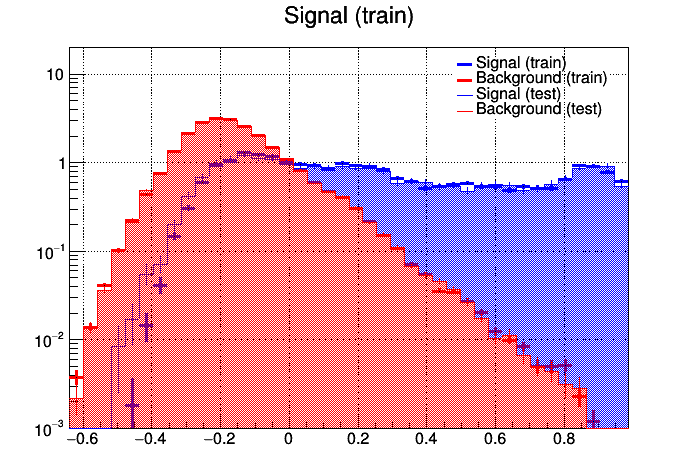
\includegraphics[width=5.2cm, height=3.5cm]{figs/log_scalar_overtraining_100GeV_TTbar_v2.png}
\end{center}
\end{minipage}
\begin{minipage}[b]{.02\textwidth}\end{minipage}
\begin{minipage}[b]{.49\textwidth}
\vspace{-5pt}
\begin{block}{\centering Pseudo 100 GeV}\end{block}
\begin{center}
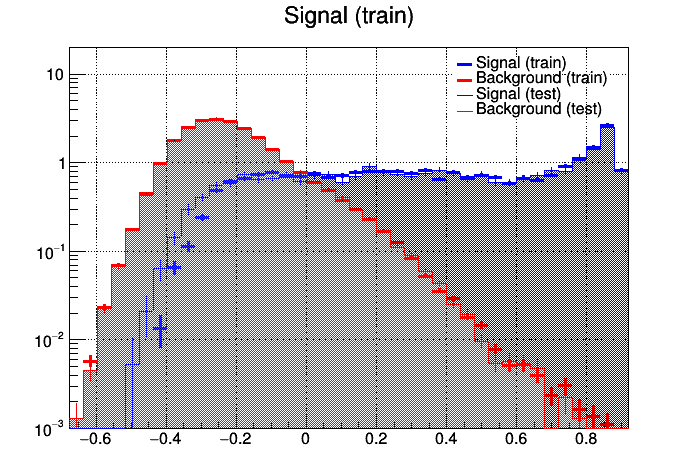
\includegraphics[width=5.2cm, height=3.5cm]{figs/log_pseudo_overtraining_100GeV_TTbar_v2.png}
\end{center}
\end{minipage}
\end{figure}

These discrepancies should not have any impact on the final results as they impact a region with very low amounts of signal. \vfill
\end{frame}








\begin{frame}{Post-fit plots (scalar 100 GeV)}
\begin{columns}
\begin{column}{1.09\textwidth}
\begin{block}{\centering $t/\bar t$+DM region (scalar 100 GeV)}\end{block} \vspace{10pt}
\end{column}
\end{columns} \vspace{-24pt}
\begin{columns}
		\begin{column}{0.33\textwidth}
			\begin{center}
			\begin{block}{\centering 2016}\end{block}	
     			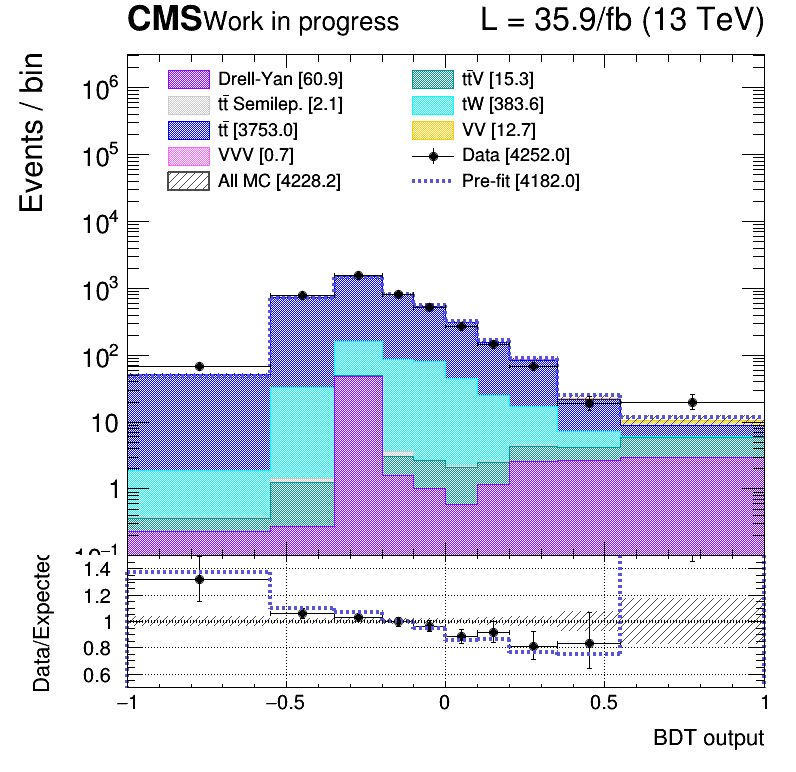
\includegraphics[width=1.0\textwidth, height=90pt]{figs/postfits/2016/log_cratio_ST_topCR_ll_BDT_tDM100_TTbar_BDT_output_scalar100_customBinsAttempt7.png}
    		\end{center}		
		\end{column} 
		\begin{column}{0.33\textwidth}
			\begin{center}
			\begin{block}{\centering 2017}\end{block}	
     			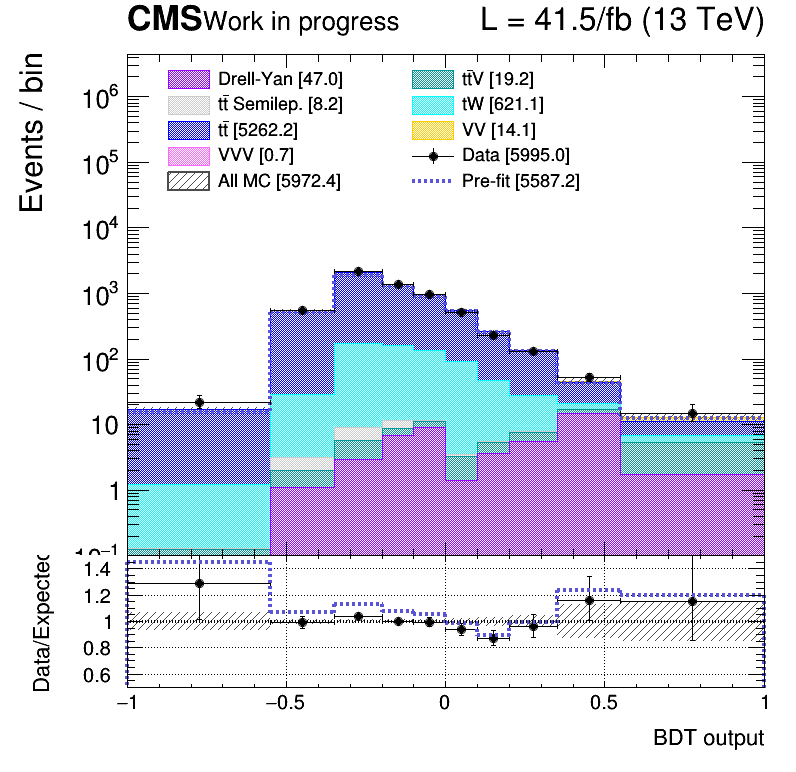
\includegraphics[width=1.0\textwidth, height=90pt]{figs/postfits/2017/log_cratio_ST_topCR_ll_BDT_tDM100_TTbar_BDT_output_scalar100_customBinsAttempt7.png}
    		\end{center}		
		\end{column} 
		\begin{column}{0.33\textwidth}
			\begin{center}
			\begin{block}{\centering 2018}\end{block}	
     			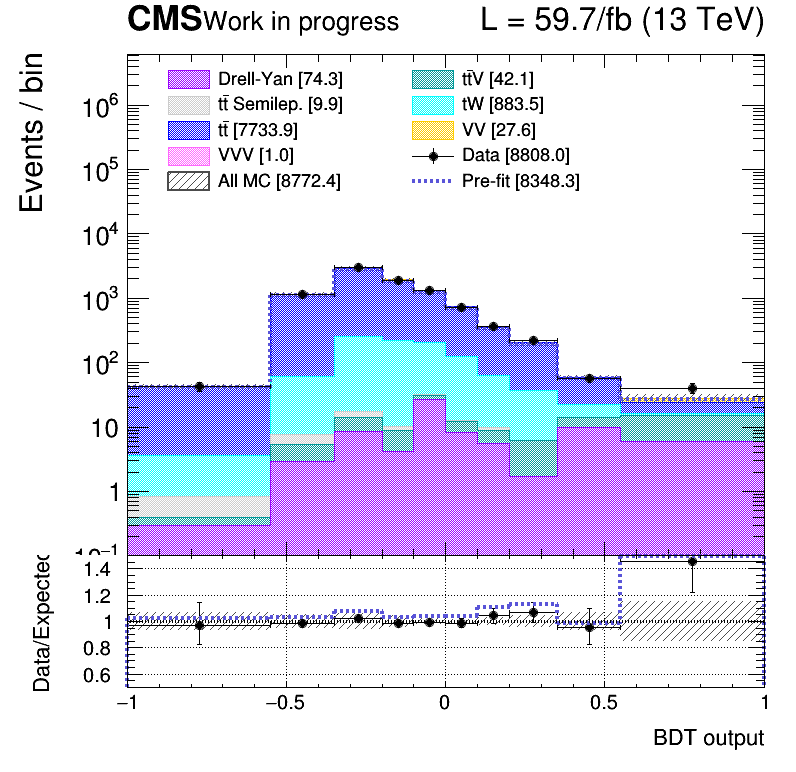
\includegraphics[width=1.0\textwidth, height=90pt]{figs/postfits/2018/log_cratio_ST_topCR_ll_BDT_tDM100_TTbar_BDT_output_scalar100_customBinsAttempt7.png}
    		\end{center}		
		\end{column}
\end{columns}

\vspace{-8pt}
\begin{columns}
\begin{column}{1.09\textwidth}
\begin{block}{\centering $t \bar t$+DM region}\end{block} \vspace{10pt}
\end{column}
\end{columns} \vspace{-16pt}
\begin{columns}
		\begin{column}{0.33\textwidth}
			\begin{center}
				%\begin{block}{\centering Puppi MET}\end{block}	
     			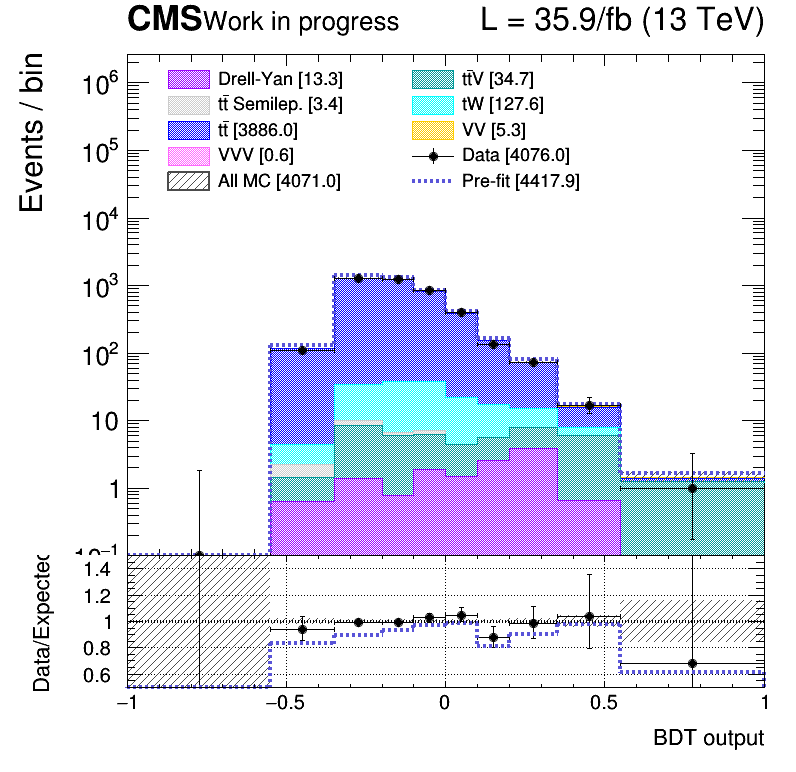
\includegraphics[width=1.0\textwidth, height=90pt]{figs/postfits/2016/log_cratio_TTbar_topCR_ll_BDT_ttDM100_TTbar_BDT_output_scalar100_customBinsAttempt7.png}
    		\end{center}		
		\end{column}
		\begin{column}{0.33\textwidth}
			\begin{center}
				%\begin{block}{\centering njet}\end{block}	
     			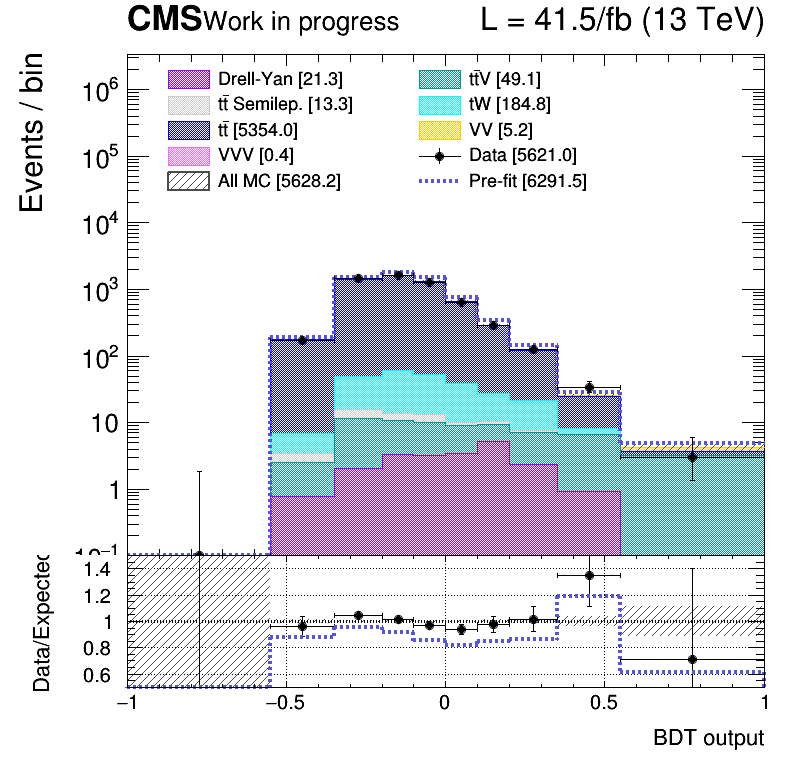
\includegraphics[width=1.0\textwidth, height=90pt]{figs/postfits/2017/log_cratio_TTbar_topCR_ll_BDT_ttDM100_TTbar_BDT_output_scalar100_customBinsAttempt7.png}
    		\end{center}		
		\end{column}
		\begin{column}{0.33\textwidth}
			\begin{center}
				%\begin{block}{\centering nbjet}\end{block}	
     			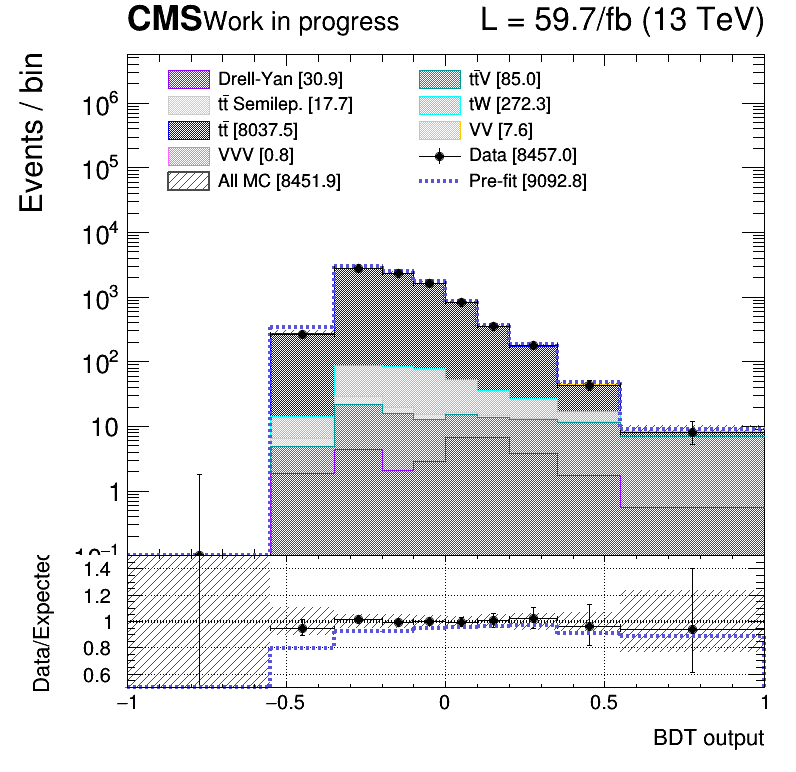
\includegraphics[width=1.0\textwidth, height=90pt]{figs/postfits/2018/log_cratio_TTbar_topCR_ll_BDT_ttDM100_TTbar_BDT_output_scalar100_customBinsAttempt7.png}
    		\end{center}		
		\end{column}
\end{columns} \vfill
\end{frame}

\begin{frame}{Post-fit plots (pseudoscalar 100 GeV)}
\begin{columns}
\begin{column}{1.09\textwidth}
\begin{block}{\centering $t/\bar t$+DM region (pseudoscalar 100 GeV)}\end{block} \vspace{10pt}
\end{column}
\end{columns} \vspace{-24pt}
\begin{columns}
		\begin{column}{0.33\textwidth}
			\begin{center}
			\begin{block}{\centering 2016}\end{block}	
     			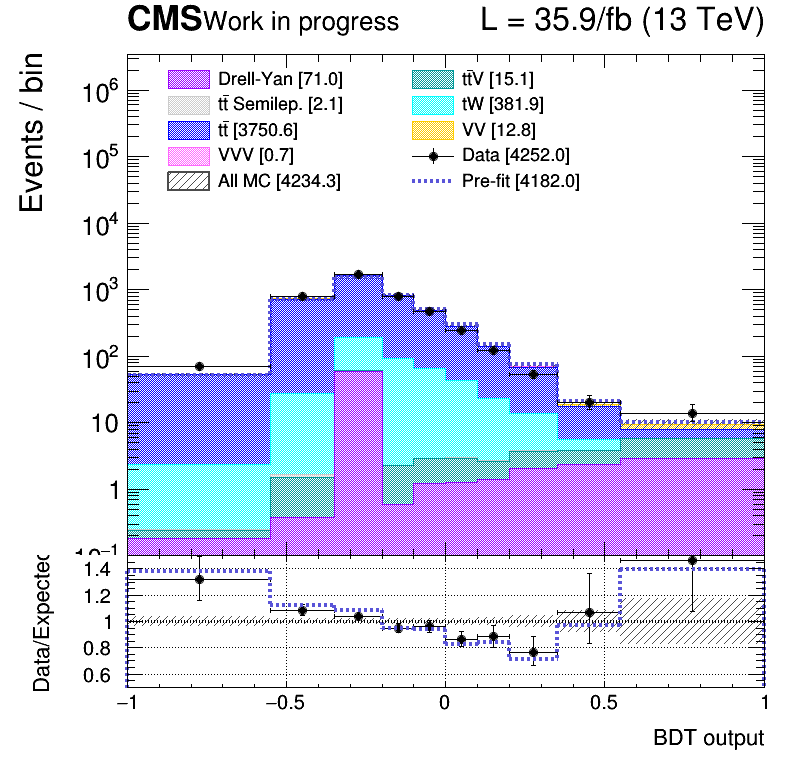
\includegraphics[width=1.0\textwidth, height=90pt]{figs/postfits/2016/log_cratio_ST_topCR_ll_BDT_tDM100_TTbar_BDT_output_pseudoscalar100_customBinsAttempt7.png}
    		\end{center}		
		\end{column} 
		\begin{column}{0.33\textwidth}
			\begin{center}
			\begin{block}{\centering 2017}\end{block}	
     			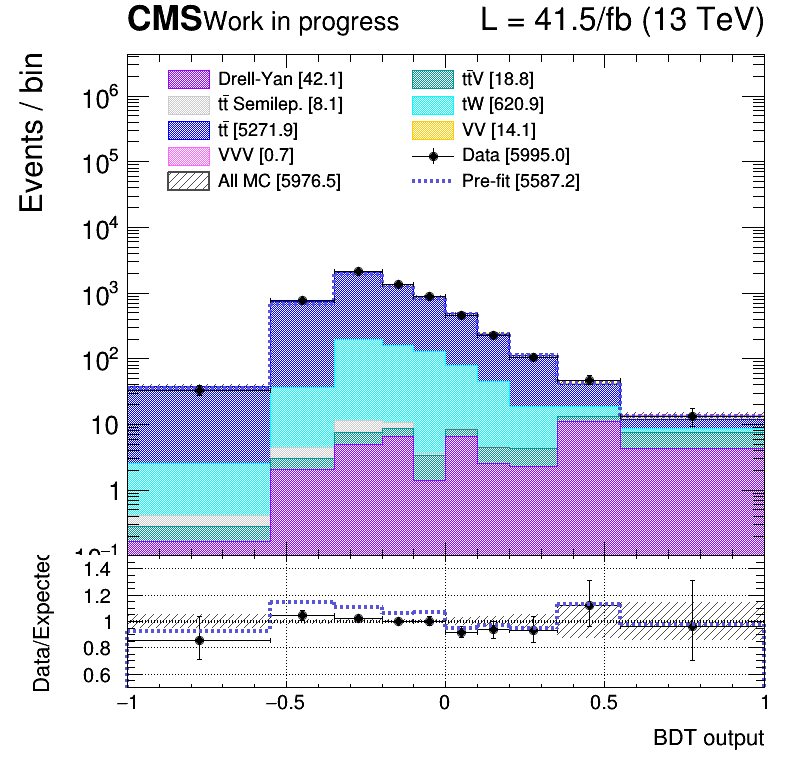
\includegraphics[width=1.0\textwidth, height=90pt]{figs/postfits/2017/log_cratio_ST_topCR_ll_BDT_tDM100_TTbar_BDT_output_pseudoscalar100_customBinsAttempt7.png}
    		\end{center}		
		\end{column} 
		\begin{column}{0.33\textwidth}
			\begin{center}
			\begin{block}{\centering 2018}\end{block}	
     			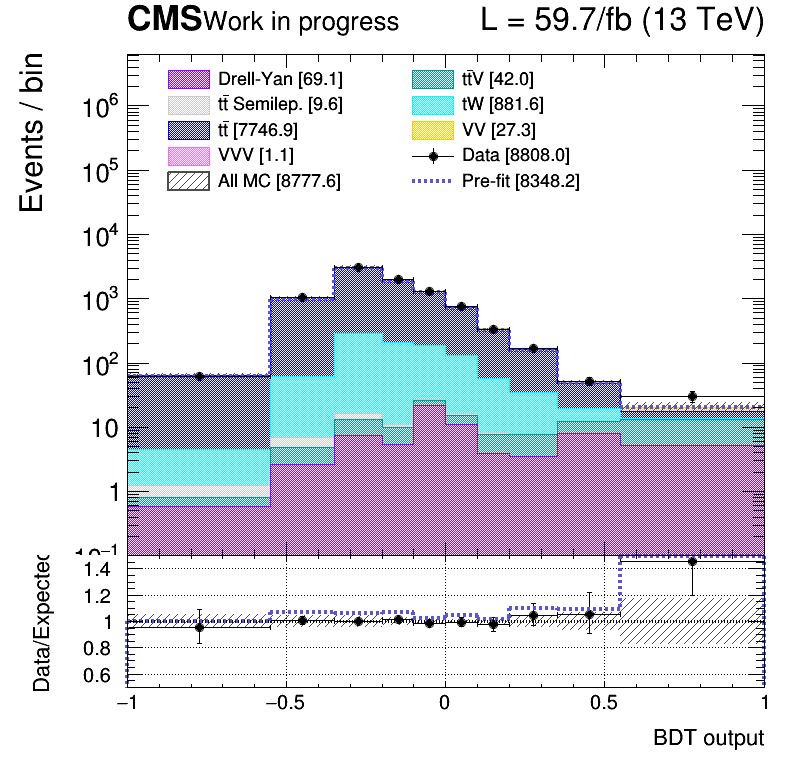
\includegraphics[width=1.0\textwidth, height=90pt]{figs/postfits/2018/log_cratio_ST_topCR_ll_BDT_tDM100_TTbar_BDT_output_pseudoscalar100_customBinsAttempt7.png}
    		\end{center}		
		\end{column}
\end{columns}

\vspace{-8pt}
\begin{columns}
\begin{column}{1.09\textwidth}
\begin{block}{\centering $t \bar t$+DM region}\end{block} \vspace{10pt}
\end{column}
\end{columns} \vspace{-16pt}
\begin{columns}
		\begin{column}{0.33\textwidth}
			\begin{center}
				%\begin{block}{\centering Puppi MET}\end{block}	
     			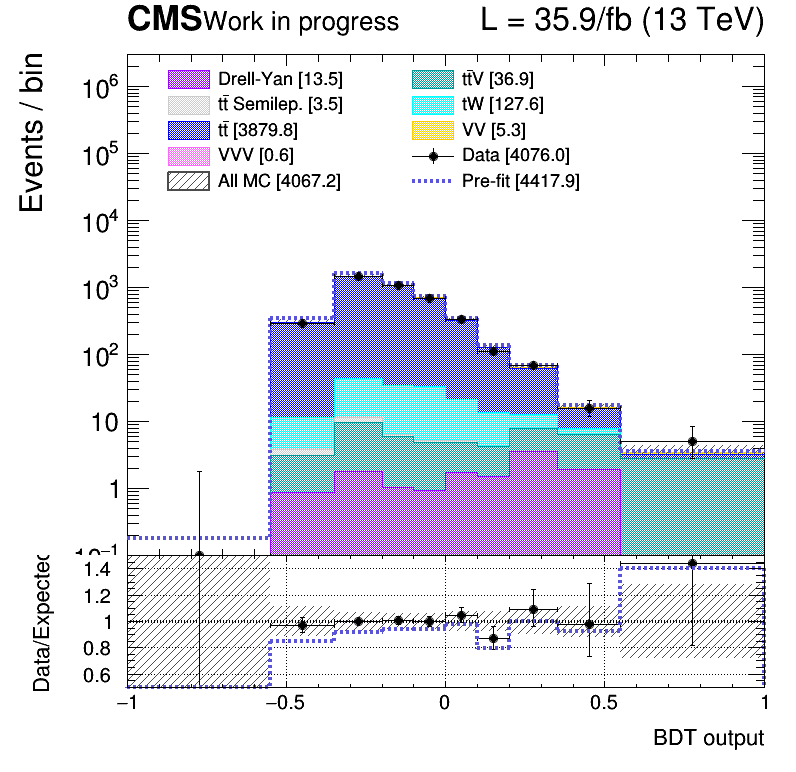
\includegraphics[width=1.0\textwidth, height=90pt]{figs/postfits/2016/log_cratio_TTbar_topCR_ll_BDT_ttDM100_TTbar_BDT_output_pseudoscalar100_customBinsAttempt7.png}
    		\end{center}		
		\end{column}
		\begin{column}{0.33\textwidth}
			\begin{center}
				%\begin{block}{\centering njet}\end{block}	
     			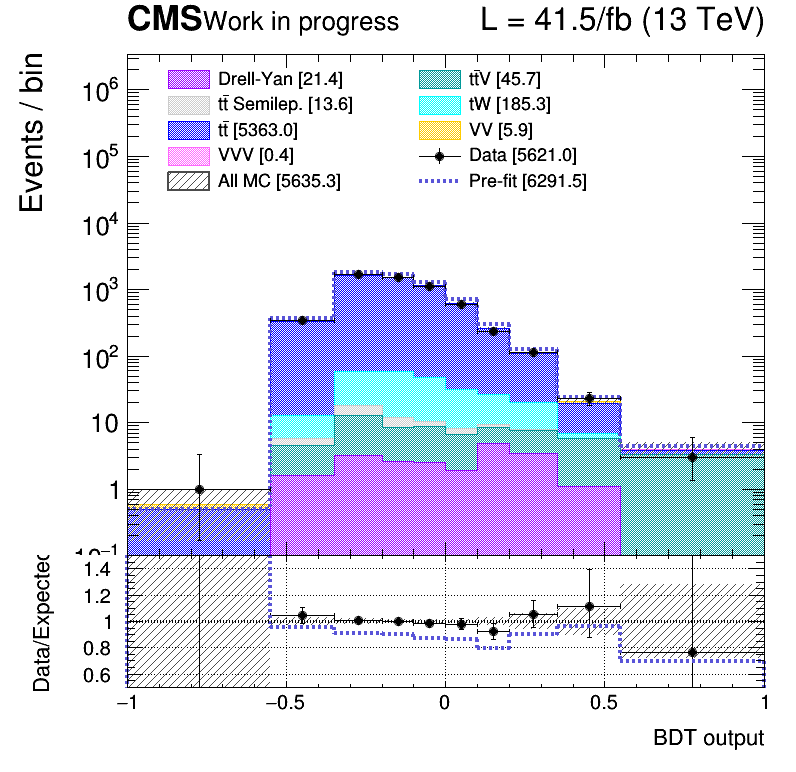
\includegraphics[width=1.0\textwidth, height=90pt]{figs/postfits/2017/log_cratio_TTbar_topCR_ll_BDT_ttDM100_TTbar_BDT_output_pseudoscalar100_customBinsAttempt7.png}
    		\end{center}		
		\end{column}
		\begin{column}{0.33\textwidth}
			\begin{center}
				%\begin{block}{\centering nbjet}\end{block}	
     			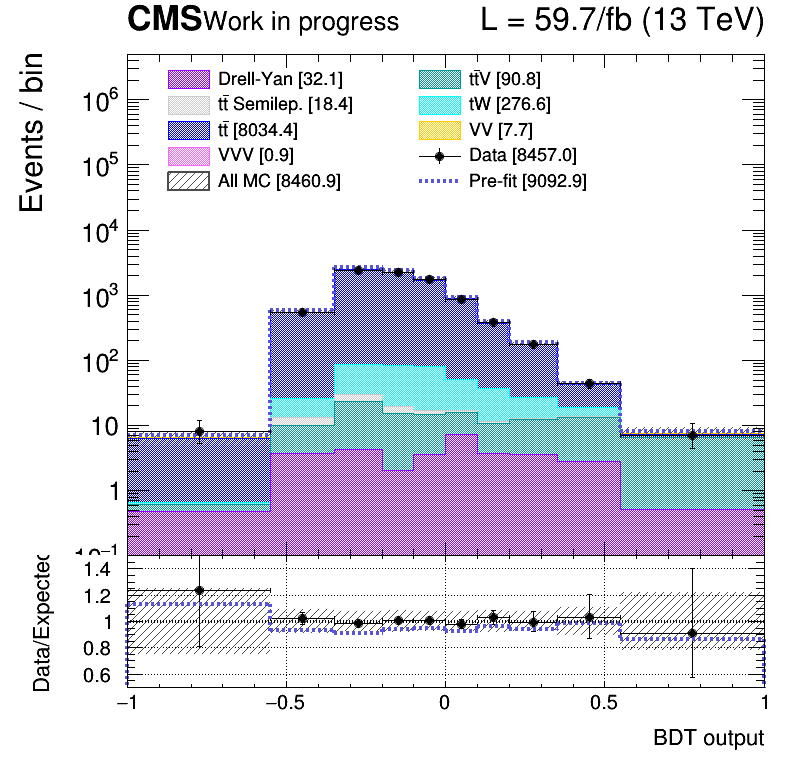
\includegraphics[width=1.0\textwidth, height=90pt]{figs/postfits/2018/log_cratio_TTbar_topCR_ll_BDT_ttDM100_TTbar_BDT_output_pseudoscalar100_customBinsAttempt7.png}
    		\end{center}		
		\end{column}
\end{columns} \vfill

All the post-fit plots can be found in the v4 of the AN-22-014. \vfill
\end{frame}


\begin{frame}{Pulls and impact plots}
\justifying
" In addition,
please provide information on the fit itself: such as pulls with the
data." \vfill

\begin{figure}[htbp]
\centering
\begin{block}{\centering 2018, scalar}\end{block}	\vspace{-8pt}

\begin{minipage}[b]{0.49\textwidth}
\begin{center}
\centering \begin{block}{\centering 100 GeV}\end{block}	
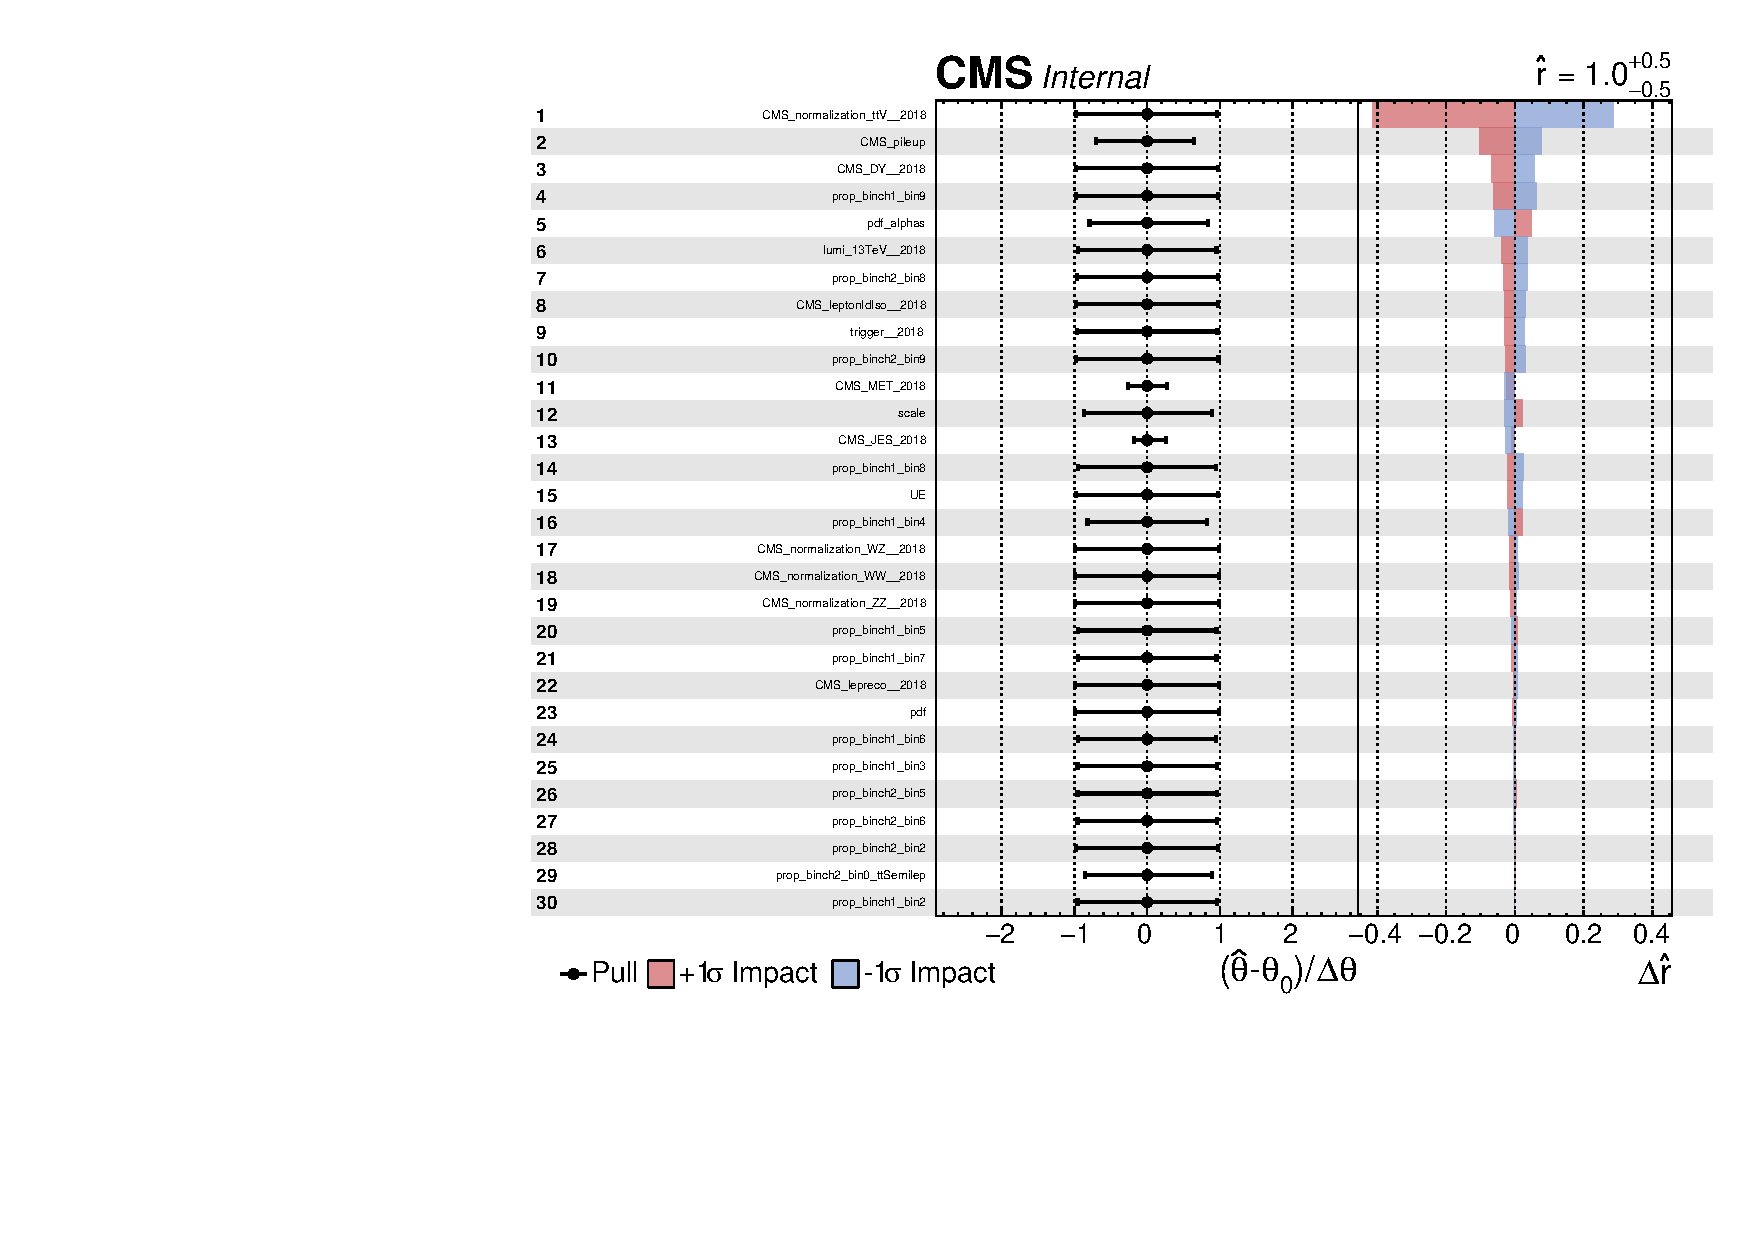
\includegraphics[width=5.1cm, height=4.2cm]{figs/impacts_2018_both_scalar_100.pdf}
\end{center}
\end{minipage}\hfill
\begin{minipage}[b]{0.49\textwidth}
\begin{center}
\centering \begin{block}{\centering 500 GeV}\end{block}	
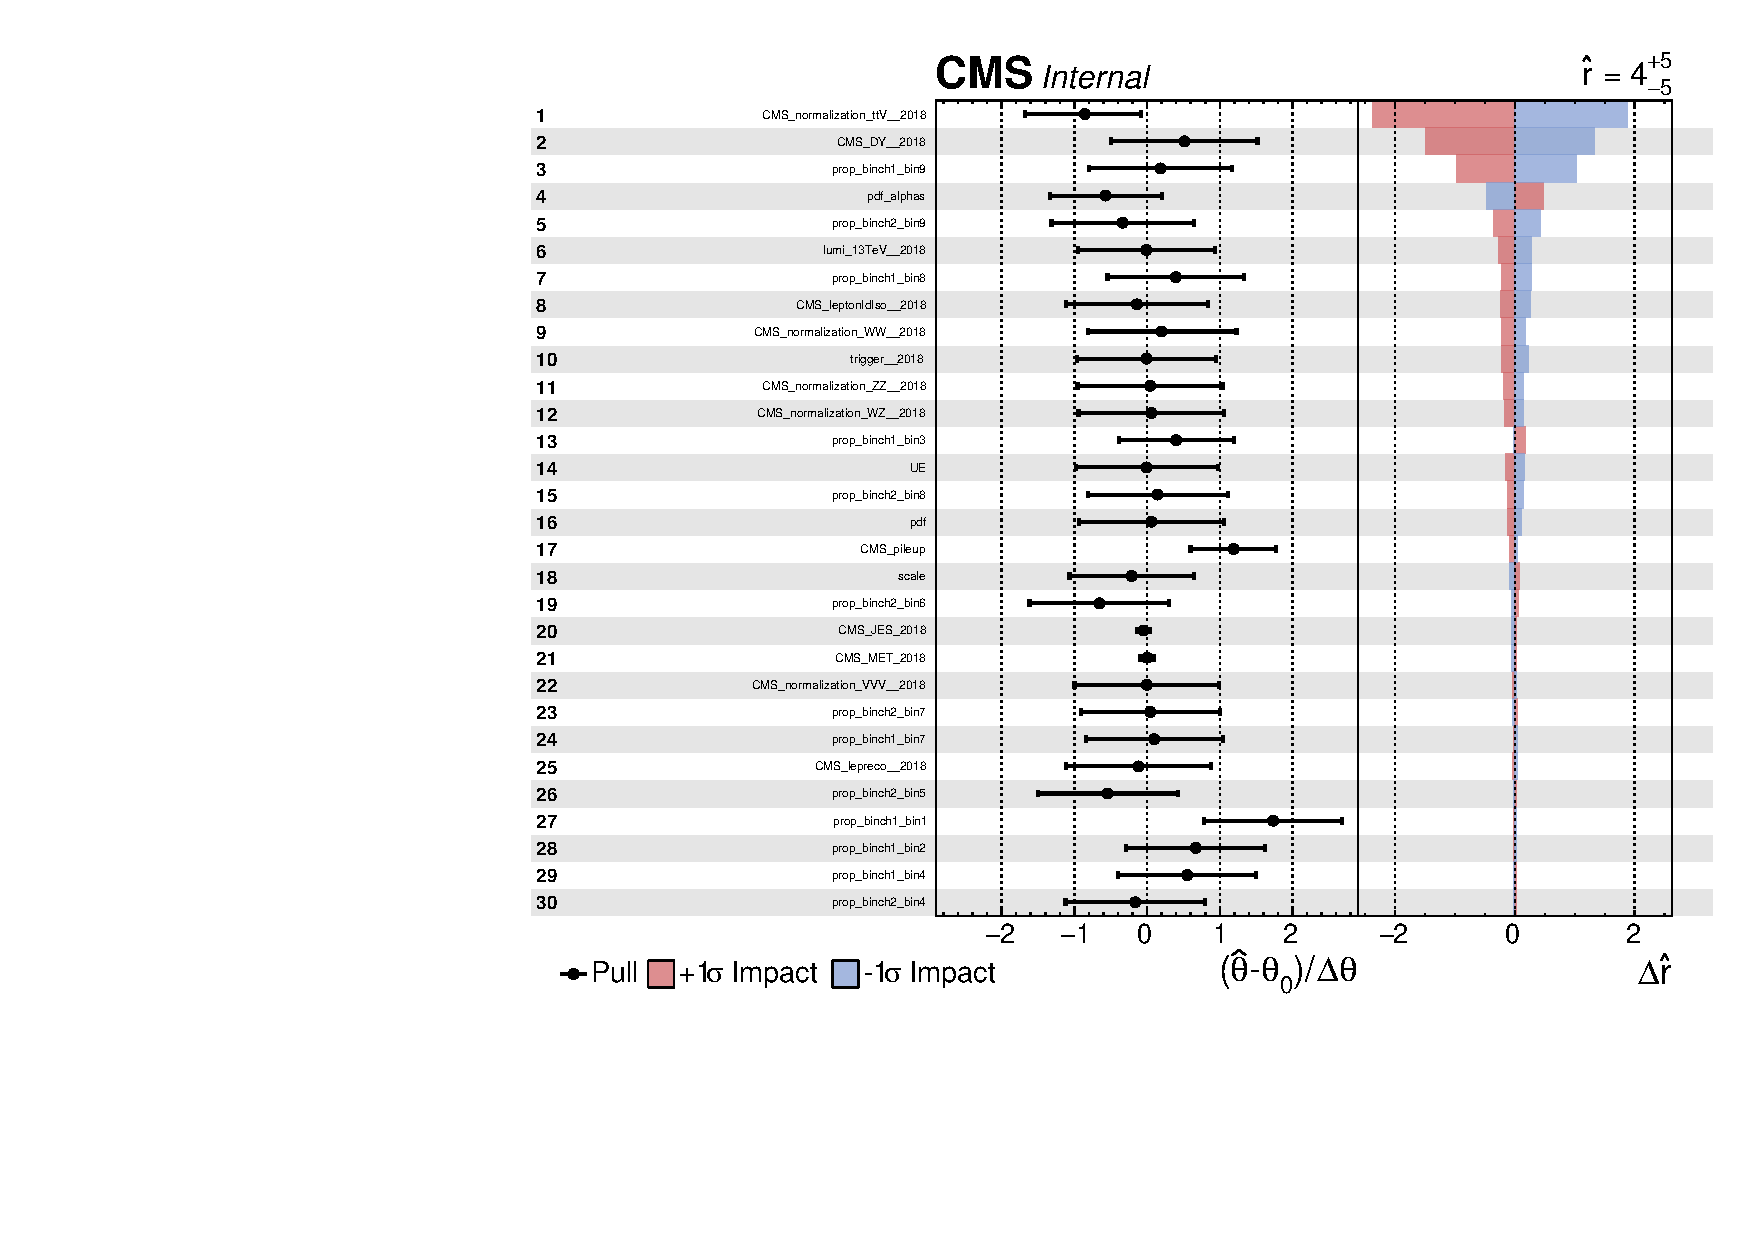
\includegraphics[width=5.1cm, height=4.2cm]{figs/impacts_2018_both_scalar_500.pdf}
\end{center}
\end{minipage} \hfill
\end{figure} \vfill

All the impact plots with real data can also be found in the newest version of the AN. In general no large pulls, the most significant effect is the constraint of the JES/MET. \vfill
\end{frame}

\begin{frame}{Pulls and impact plots}
\justifying
%These strong constraints seem to come from the low BDT output region of the plots fed into the algorithm, where a lot of $ \bar t$ can be found. This region might actually play the role of a $t \bar t$ control region, therefore constraining a lot these two systematic. \vfill
%We therefore tried removing the BDT output $< 0$ region, getting results less constrained. \vfill

These strong constraints seem to come from the low BDT output region of the plots
fed into the algorithm, where a lot of $t \bar t$ can be found. This region is playing
the role of a control region constraining a lot these two systematics. \vfill
We therefore tried removing the BDT output $< 0$ region and observed that the constraints were gone. \vfill

\begin{figure}[htbp]
\centering
\begin{block}{\centering 2018, scalar}\end{block}	\vspace{-8pt}

\begin{minipage}[b]{0.49\textwidth}
\begin{center}
\centering \begin{block}{\centering 100 GeV}\end{block}	
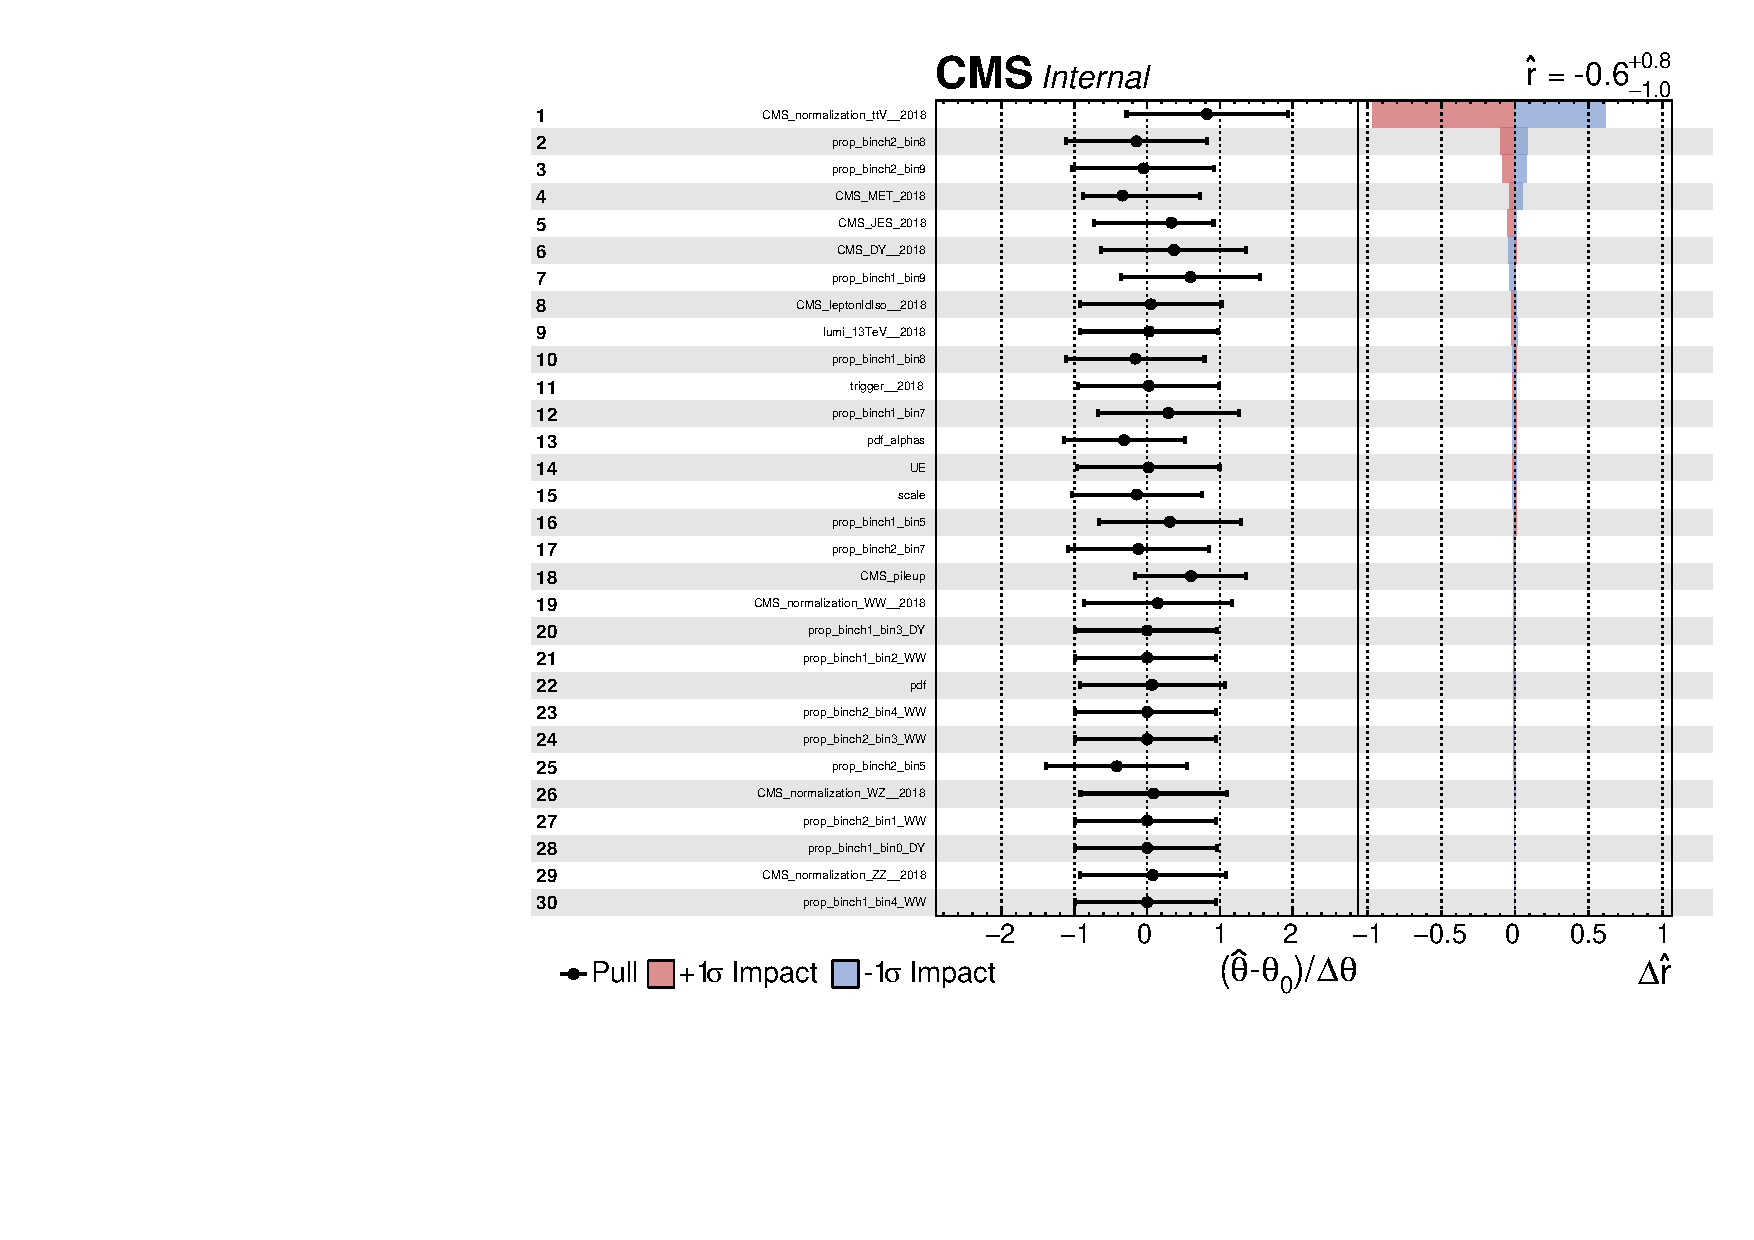
\includegraphics[width=5.1cm, height=4.2cm]{figs/impacts_fixed/impacts_2018_both_scalar_100.pdf}
\end{center}
\end{minipage}\hfill
\begin{minipage}[b]{0.49\textwidth}
\begin{center}
\centering \begin{block}{\centering 500 GeV}\end{block}	
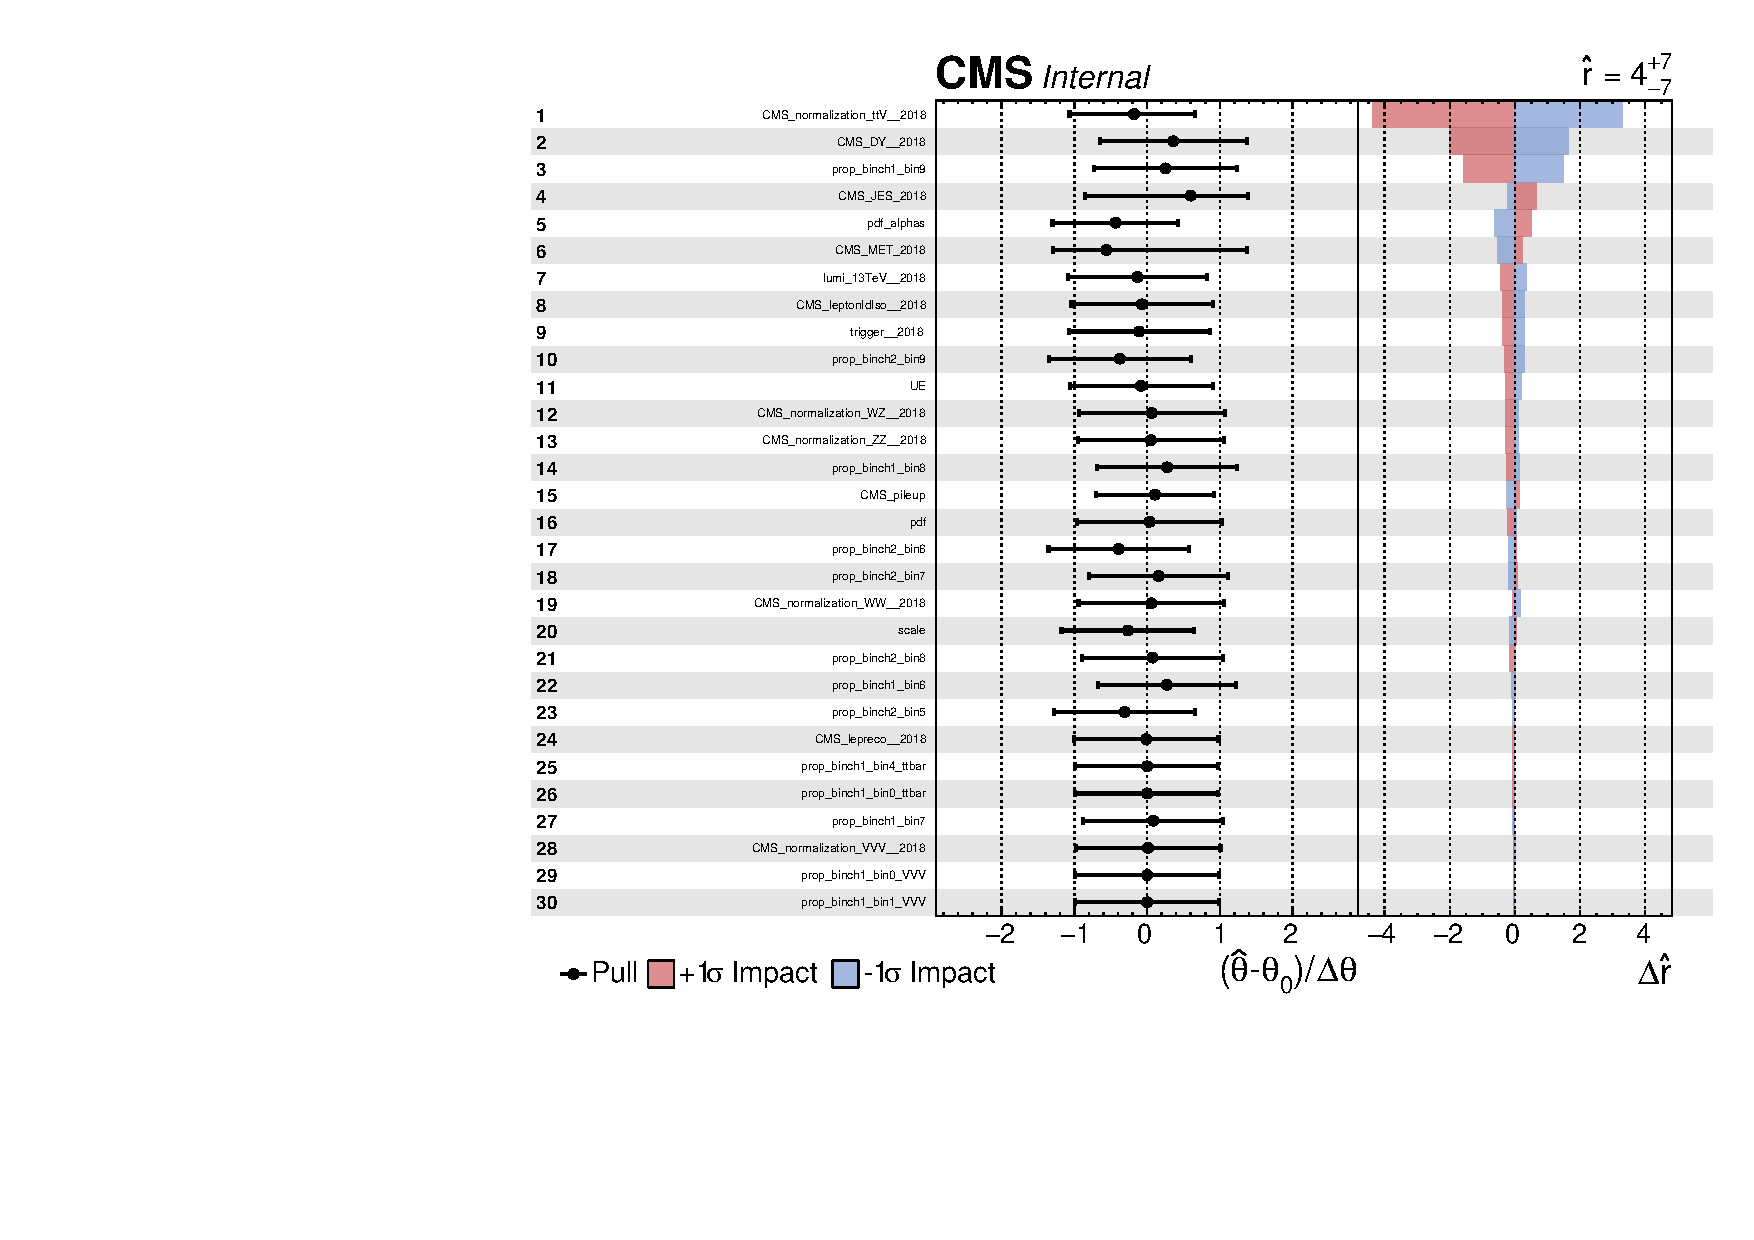
\includegraphics[width=5.1cm, height=4.2cm]{figs/impacts_fixed/impacts_2018_both_scalar_500.pdf}
\end{center}
\end{minipage} \hfill
\end{figure} \vfill
\end{frame}

\end{document}
